\documentclass[]{mgr}

\usepackage{polski}

\usepackage[utf8]{inputenc}
\usepackage[T1]{fontenc}

\usepackage{graphicx}
\usepackage{caption}
\usepackage{subcaption}

\usepackage{wrapfig}
\usepackage{psfrag}

\usepackage{amsmath}
\usepackage{amsfonts}

\usepackage{listings}
\usepackage{url}

\title{System ekspertowy dopasowujący wskazania systemu DXCluster do potrzeb użytkowników}
\engtitle{Expert system for matching DXCluster system to identify the needs of users}
\author{Paweł Marcin Szwagierek}
\supervisor{dr inż. Jerzy Greblicki, I-6}
\date{2015}

\field{Informatyka (INF)}
\specialisation{Inżynieria Internetowa (INT)}

\makeatletter
\def\@makechapterhead#1{%
  \vspace*{50\p@}%
  {\parindent \z@ \raggedright \normalfont
    \ifnum \c@secnumdepth >\m@ne
      \if@mainmatter
        \Huge\bfseries \thechapter.\space%
      \fi
    \fi
    \interlinepenalty\@M
    \Huge \bfseries #1\par\nobreak
    \vskip 40\p@
  }}
\makeatother

\begin{document}
    \bibliographystyle{plabbrv}
    \maketitle

    \tableofcontents

    \chapter{Problematyka amatorskich systemów radiowych}
    \label{sec:teoretical_description}
    W pierwszym rozdziale zostaną wprowadzone podstawowe pojęcia z dziedziny krótkofalarstwa, jego możliwości, zakres działań radioamatorów.

        \section{Radioamator}
        Cała dziedzina krótkofalarstwa nie miałaby sensu gdyby nie amatorzy zafascynowani radiokomunikacją, pasjonaci łączności lokalnych oraz łączności dalekiego zasięgu a także naukowcy i specjaliści ciągle udoskonalający istniejące projekty. W ogromnej większości radioamatorzy to osoby zajmujące się radiotechniką niezawodowo. Istnieją radioamatorzy bierni, poprzestający na studiowaniu samego tematu krótkofalarstwa, rzadko wkraczający w~dziedzinę praktyki radioamatorskiej. Amatorzy czynni na podstawie zezwolenia odpowiednich władz budują i~uruchamiają własne, indywidualnie lub zbiorowo (działając w~różnego rodzaju klubach), krótkofalowe i~ultrakrótkofalowe stacje nadawcze małej mocy.

        Duża część pracy radioamatora to próby, eksperymenty, budowanie swoich projektów a następnie wymiana doświadczeń z innymi. Zwykle są to wnioski na podstawie krótkich obserwacji, lecz niejednokrotnie są to duże i konkretne artykuły prezentowane w czasopismach branżowych. Wymieniane są spostrzeżenia dotyczące techniki radioamatorskiej, rozprzestrzeniania się fal elektromagnetycznych w~poszczególnych zakresach itp. Często w ten sposób społeczność radioamatorów przyczynia się do rozwoju wiedzy i~techniki. 

        \section{Krótkofalarstwo}
        Terminem krótkofalarstwo określa się hobby polegające na nawiązywaniu łączności z~innymi stacjami radioamatorskimi za pomocą nadajników radiowych. W~przypadku nowoczesnych sposobów komunikacji (np. poczta elektroniczna, komunikatory Internetowe, telefonia komórkowa), nieważny jest sposób przesłania informacji z~punktu A do punku~B, a sama informacja. W wypadku krótkofalarstwa większy nacisk kładzie się na sposób przesłania informacji (sprzęt radiowy, rodzaj emisji, pasmo, anteny itd) a także w wielu przypadkach na sam fakt przeprowadzonej łączności dalekiego dasięgu. Łączność ze stacją, która jest aktywna przykładowo jednego losowego dnia w roku może być bardzo dużym wyzwaniem. Podczas samych łączności krótkofalarskich istotnymi informacjami wymienianymi przez użytkowników stacji są ich osobiste znaki wywoławcze oraz raporty o~słyszalności i~sile odebranego sygnału, a~także wykorzystanych antenach, radioodbiornikach, programach komputerowych użytych do wykorzystania modulacji cyfrowych i innych parametrach związanych z~aktualnie przeprowadzaną łącznością. Samo krótkofalarstwo jest dziedziną zainteresowań o~bogatym wachlarzu możliwości.

            \subsection{Edukacja}
            (!!! COPIED !!!) Jednym z~korzyści jakie niesie ze sobą ten temat, to ogromna ilość wiedzy z~różnych lecz poniekąd pokrewnych sobie dziedzin. Taka wiedza może zostać przekazana uczniom szkół w~czasie zajęć obejmujących zagadnienia ściśle powiązane z~krótkofalarstwem. Bogatą wiedzę można także pozyskać uczestnicząc w~spotkaniach klubów krótkofalarskich lub uczestnicząc w~zajęciach prowadzonych przez takie kluby. Przekazywane tam informacje są najbardziej usystematyzowane. Rozwiązanie takie daje także możliwości skorzystania z~klubowych radiostacji. Ostatnim ze sposobów podjęcia takiej wiedzy jest nauka samodzielna korzystając z~rozmaitej literatury tematycznej, publikacji lub artykułów sporządzonych samodzielnie przez radioamatorów z~całego świata.

            Przede wszystkim radioamator uczy się przy okazji pasji dużo z~dziedziny telekomunikacji. Poznaje rodzaje anten, które wykorzystuje się w~pracy z~różnymi pasmami a także ich budowę. Uczy się także typów modulacji oraz rodzajów emisji. W~przypadku elektroniki krótkofalarstwo daje szansę poznania zasad działania różnych urządzeń elektronicznych oraz zagadnienia przetwarzania sygnałów. Budowanie automatycznych przełączników lub sterowników rotorów antenowych wiąże się z~poznaniem zagadnień z~dziedziny automatyki. Krótkofalarstwo wprowadza także wiele wiedzy z~zakresu informatyki, gdzie radioamator może wykorzystać do transmisji informacji różne rodzaje emisji cyfrowych lub stworzyć swój własny system SDR\footnote{SDR (ang. Software Defined Radio, radio programowalne) – system komunikacji radiowej, w~którym działanie podstawowych elementów elektronicznych (takich jak mieszacze, filtry, modulatory i~demodulatory) jest realizowane za pomocą programu komputerowego.} i~korzystać ze swojego oddalonego o~znaczną odległość radia za pośrednictwem Internetu lub dać możliwość korzystania ze swoich anten i~prowadzenia nasłuchu innym radioamatorom. Na pograniczu leżą także takie dziedziny nauki jak kryptografia, w~przypadku gdy użytkownicy dwóch stacji chcą się porozumiewać zachowując poufność przesyłanych informacji. Istotną umiejętnością jest także znajomość języków obcych. Bez tego prawie niemożliwym jest prowadzenie łączności z~radioamatorami posługującymi się innymi językami. Krótkofalarstwo wprowadza także wiele umiejętności stricte powiazanych z tą dziedziną - umiejętność komunikacji za pomocą telegrafii (alfabetem Morse'a), znajomość fonetycznej reprezentacji liter w różnych językach (\mbox{A -- Alpha/Adam}, B -- Bravo/Barbara, C -- Charlie/Celina, itd.).

            Jest to jedna z~nielicznych pasji, która pozwala na wykorzystanie w globalnych łącznościach własnoręcznie stworzonego sprzętu. Społeczność krótkofalowców popiera i~wręcz dopinguje budowanie i~wykorzystanie własnych urządzeń radiowych, anten a także pozostałego oprzyrządowania niezbędnego w~pracy lub ułatwiającego pracę radioamatora - jak na przykład przełączniki antenowe, wzmacniacze, klucze telegraficzne itp) oraz programów komputerowych - do transmisji danych różnymi typami emisji, do monitorowania pracy radioamatora lub do sterowania pracą radioodbiornika za pomocą komputera. Dodatkowym atutem jest brak konieczności posiadania jakichkolwiek homologacji lub zezwoleń na korzystanie z~własnych urządzeń, co jest ogromną zaletą w przeciwieństwie do pasm CB, gdzie urządzenie musi być homologowane i mieć określone warunki pracy lub pasm PMR (w jakich pracują na przykład proste urządzenia Walkie-Talkie), gdzie urządzenie musi być o bardzo niskiej mocy, mieć na stale przyczepioną antenę i trwale zamkniętą obudowę aby uniemożliwić ingerencję ze strony użytkowników. Najwięcej osób używa jednak urządzeń fabrycznych. Jest to droższe rozwiązanie, ale dużo łatwiejsze aby od razu zacząć komunikację z innymi.

            \subsection{Amatorska Służba Radiowa}
            Radioamatorzy posiadający urządzenia nadawczo-odbiorcze są w~stanie skomunikować się ze znaczną grupą osób w~swoim otoczeniu lub dowolnym zakątkiem kraju czy świata. To daje możliwość pomocy innym ludziom w~wymianie informacji w~sytuacjach nieprzewidzianych, nagłych wypadkach, katastrofach lub klęskach żywiołowych. Krótkofalowcy są często jedynymi, którym udaje się nawiązać łączność pomiędzy odciętymi komunikacyjnie regionami. Najlepszym przykładem może tu być przypadek powodzi jaka nawiedziła województwa Dolnośląskie oraz Opolskie w 1997 roku. Z powodu braku zasilania i awarii tradycyjnych metod komunikacji większość informacji pomiędzy ludnością cywilną przekazywana była dzięki pracy krótkofalowców. Informacje o zagnionych lub znalezionych osobach, o~stanie wody lub nadchodzących nowych zagrożeniach. Krótkofalowcy pomagali również podczas powodzi w 2007 i 2010 roku.

            Wielu radioamatorów angażuje się także w~szkolenie innych ludzi w~zakresie krótkofalarstwa lub dziedzin ściśle z~nim powiązanych. To nieoceniona pomoc dla początkujących, która pozwala łatwiej zacząć przygodę z~krótkofalarstwem i wdrożyć się tematykę bez konieczności czytania wielu potężnych tomów literatury lub czasopism branżowych.

            \subsection{Hobby}
            (!!! COPIED !!!) Najwięcej ludzi skłania się do krótkofalarstwa z~powodu hobby. Posiada wiele dyscyplin jak zawody, wyprawy, prowadzenie łączności dalekiego zasięgu, eksperymentowanie z~różnymi typami emisji lub po prostu pozostawanie w~kontakcie z~przyjaciółmi korzystając z~innego środka komunikacji od popularnych w~dzisiejszych czasach telefonii komórkowej czy Internetu.

                \subsubsection{Zawody}
                    \begin{wrapfigure}{r}{0.4\textwidth}
                        \vspace{-25pt}
                        \begin{center}
                            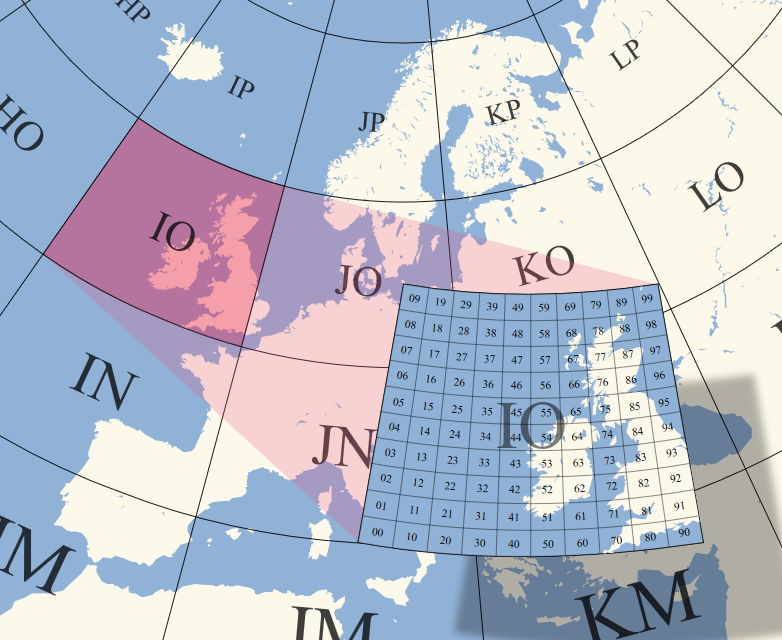
\includegraphics[scale=0.20]{gridsquare}
                        \end{center}
                        \vspace{-20pt}
                        \caption{Podział ziemi na kwadraty do określenia lokatora stacji}
                        \vspace{-10pt}
                        \label{fig:gridsquare}
                    \end{wrapfigure}
                Jedną z~dziedzin rywalizacji pomiędzy radioamatorami są zawody przeprowadzane w~ściśle określonym czasie. Polegają na nawiązaniu jak największej liczby łączności z~innymi operatorami stacji i~tym samym zdobywaniu punktów przydzielanych według zasad określonych w~regulaminie. Zaliczane są tylko bezbłędne łączności potwierdzone wymienionymi znakami wywoławczymi, raportami RST\footnote{RST (Readability, Strength, Tone) - raport oceniający Czytelność, Siłę oraz Ton aktualnie odbieranego sygnału. Składa się z trzech składowych, z których pierwsza (czytelność) oceniana jest w skali 1-5, druga (siła sygnału) w skali 1-9 i trzecia (ton - nieużywana w przypadku łączności fonicznych) w~\mbox{skali~1-9}. Najczęstszymi raportami są raporty 59 określające doskonałą czytelność odbieranych komunikatów i mocną siłę sygnału}, numerami porządkowymi łączności oraz lokatorami\footnote{Lokator - (ang. Grid Square Locator) – System Lokatorów, w którym świat jest podzielony na równe kwadraty. Każdy z kwadratów jest podzielony na kolejne itd. (rys.~\ref{fig:gridsquare}). Pozycja geograficzna jest zapisywana w formacie LLCCLL - gdzie L to litera a C to cyfra. Dla przykładu lokator gmachu głównego Politechniki Wrocławskiej to JO81MC.} swojej stacji. Te dane po zakończeniu zawodów poddawane są weryfikacji przez organizatora przy pomocy programów komputerowych. Zwykle nagrodami są dyplomy dla osoby lub drużyny wygrywającej zawody.

                \subsubsection{Łączności lokalne}
                    \begin{wrapfigure}{r}{0.4\textwidth}
                        \vspace{-20pt}
                        \begin{center}
                            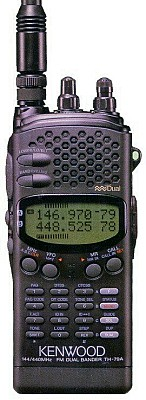
\includegraphics[scale=0.5]{ukf_handheld}
                        \end{center}
                        \vspace{-20pt}
                        \caption{Prosty nadajnik ręczny do pracy w~paśmie UKF}
                        \vspace{-20pt}
                        \label{fig:ukf_handheld}
                    \end{wrapfigure}
                Do prowadzenia łączności ze znajomymi mieszkającymi w~naszym otoczeniu wystarczy tani nadajnik przenośny, jak pokazany na rysunku~\ref{fig:ukf_handheld} lub samochodowy pracujący na pasmach UKF. Stosunkowo mała moc urządzeń pozwala na objęcie swoim zasięgiem czasami nawet całego miasta. W~przypadku gdy taki zasięg staje się niewystarczający, w~orężu radioamatorów pozostają tzw. przemienniki - urządzenia montowane na znacznych wysokościach (wysokich obiektach miejskich, wzniesieniach terenu), które odbierają sygnał i~nadają go powtórnie z~dużo większą mocą. Skutkuje to wielokrotnym zwiększeniem zasięgu prowadzonych łączności nawet do kilkuset kilometrów. Przemienniki amatorskie nie nadają cały czas, aby nie zużywały energii gdy nikt z~nich nie korzysta. W~celu skorzystania z~takiego przemiennika należy go wcześniej ,,otworzyć'' sygnałem akustycznym o~określonej częstotliwości, jednym z~tonów DTMF lub sygnałów CTCSS.

                \subsubsection{Łączności dalekiego zasięgu (DX)}
                (!!! Copied !!!) Radioamatorzy, którzy korzystają z~bardziej zaawansowanych urządzeń i~anten mogą pracować z~innymi rodzajami emisji oraz na innych pasmach (fale krótkie (KF), fale średnie). Pozwala to na realizację łączności na dużo większe odległości - opierając się na samej mocy i~charakterystyce emitowanego sygnału, wykorzystując zjawiska pogodowe, zjawisko odbicia fal lub korzystając z~amatorskich satelitów komunikacyjnych działających w~paśmie UKF. Można dzięki temu nawiązywać łączności międzykontynentalne na dystansach rzędu tysięcy kilometrów.

                    \paragraph{Fale odbite od warstw jonosfery}
                    Łączności dalekiego zasięgu na falach krótkich można zrealizować korzystając z~nadajników małej mocy i~nieskomplikowanych drutowych anten wykorzystując zjawisko odbicia fal od jonosfery. Zjawisko to występuje powszechnie i~w~zależności od pory dnia i~aktywności słonecznej umożliwia łączności na odległość od kilkuset do kilkunastu tysięcy kilometrów. Łączności z~najbardziej odległymi stacjami prowadzi się poprzez wielokrotne odbicia, niekiedy pokonujące dłuższą drogę wokół kuli ziemskiej.

                    \paragraph{Fale odbite od powierzchni księżyca}
                    Jednym z~najbardziej niezwykłych rodzajów łączności są te z~wykorzystaniem odbicia fali od powierzchni księżyca (EME). Do tego typu łączności wykorzystuje się zaawansowane systemy antenowe (jak przedstawiona na rysunku~\ref{fig:eme_antenna} oraz nadajniki o~wysokiej mocy. Przy EME wymagana jest duża precyzja oraz doświadczenie w~prowadzeniu takich łączności, przez co jest to dziedzina krótkofalarstwa która odstrasza początkujących radioamatorów. 

                    Antena powinna być skierowana dokładnie w~kierunku księżyca, który pozostaje w~ruchu względem powierzchni ziemi. W~związku z~tym aby powszechnie wykorzystywanymi są skomplikowane systemy obracania anten. W~przypadku złego ustawienia anteny najczęstszymi zakłóceniami sygnału są zniekształcenia czoła fali w~wyniku nakładania się fal odbitych. Typowymi dla tego rodzaju łączności są zjawiska odbioru własnego echa po około 2 sekundach od wysłania komunikatu oraz niewyjaśnione dotąd echo z~dużym opóźnieniem. Skutkiem tego jest otrzymanie przez nadawcę swojego komunikatu ale po czasie dochodzącym nawet do kilku minut.

                        \begin{wrapfigure}{r}{0.4\textwidth}
                            \vspace{-20pt}
                            \begin{center}
                                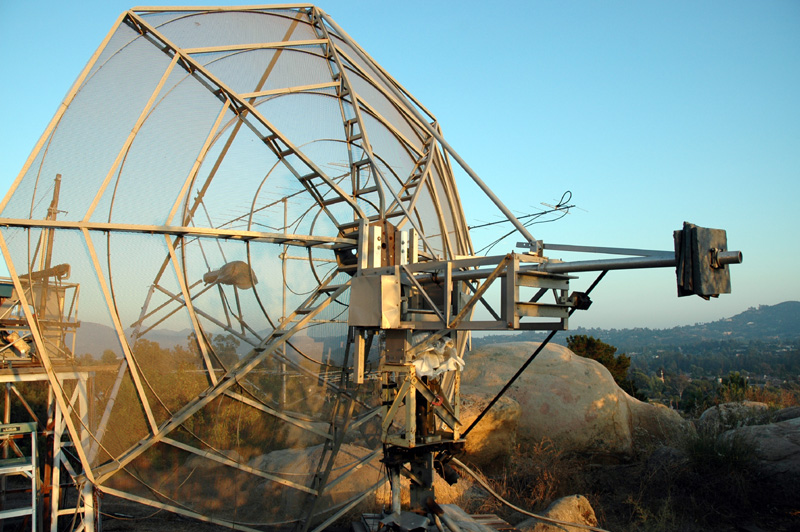
\includegraphics[width=0.4\textwidth]{eme_antenna}
                            \end{center}
                            \vspace{-20pt}
                            \caption{Antena paraboliczna wykorzystywana do łączności EME pracująca w~paśmie fal 430MHz}
                            \vspace{-20pt}
                            \label{fig:eme_antenna}
                        \end{wrapfigure}

                    Łączności wykonywane tą techniką ze względu na małą skuteczność, małą pewność transmisji oraz trudności związane z~jej wykonaniem realizują tylko radioamatorzy.

                    \paragraph{Łączności satelitarne}
                    Krótkofalowcy korzystają także ze swoich satelitów. Takich satelitów niskoorbitalnych\footnote{Satelita niskoorbitalny - satelita krążący wokół Ziemi po orbicie kołowej na wysokości 10 tys. km - 500 tys. km} jest kilkadziesiąt i~co jakiś czas wysyłane są kolejne. Fale pasma UKF pozwalają na przeprowadzenie łączności z~astronautami z~międzynarodowej stacji kosmicznej ISS a także na łączności pomiędzy radioamatorami. Korzystanie z~satelitów wymaga znajomości ich pozycji na niebie, parametrów pracy oraz ciągłego korygowania ustawienia anteny. Także sama komunikacja wygląda nieco inaczej niż w~przypadku normalnej łączności. W~przypadku satelity wiadomości nadawane są na częstotliwości zwanej ,,uplink'' i~odbierane na częstotliwości oznaczonej jako ,,downlink''. Jest to uwarunkowane zasadą pracy satelity. Odbiera ona sygnały z~jednej częstotliwości i~retransmituje te same sygnały ze zwiększoną mocą na innej częstotliwości - podobnie jak to dzieje się w~przypadku przemienników amatorskich.
                        \begin{wrapfigure}{r}{0.4\textwidth}
                            \vspace{-25pt}
                            \begin{center}
                                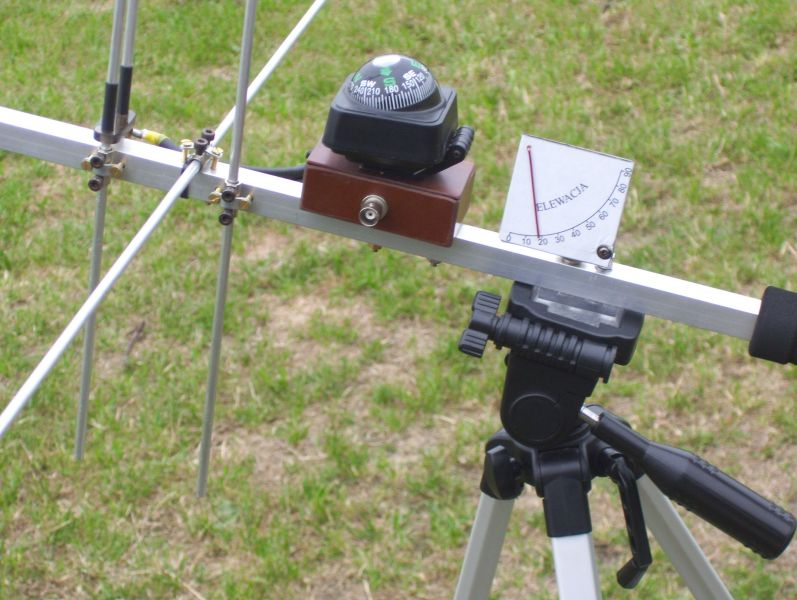
\includegraphics[width=0.4\textwidth]{example_sat_construction}
                            \end{center}
                            \vspace{-20pt}
                            \caption{Konstrukcja radioamatora SQ5RJK do ręcznego ustawiania i~korygowania pozycji anteny podczas łączności satelitarnych}
                            \vspace{-50pt}
                            \label{fig:example_sat_construction}
                        \end{wrapfigure}
                    W~związku z~tym, że pozycja anteny musi być na bieżąco korygowana, stosuje się skomplikowane systemy obracania anten lub rolę tę przejmuje sam radioamator i~pozycję anteny koryguje ręcznie korzystając z~takich konstrukcji jak pokazana na rysunku~\ref{fig:example_sat_construction}.

                    \paragraph{Inne typy łączności}
                    Sporadycznie radioamatorzy korzystają do zrealizowania łączności z~takich zjawisk jak odbicia fal radiowych od zorzy polarnej, meteorytów a nawet chmur burzowych.

                \subsubsection{Wyprawy}
                (!!! Copied !!!) W~społeczności krótkofalarskiej popularnymi są także wyprawy zwane inaczej DXpedycjami. Radioamatorzy w~pojedynkę lub w~zorganizowanej grupie wraz z~członkami klubu zdobywają górę lub niezamieszkały teren aby tam utworzyć tymczasową stację i~przeprowadzić łączności z~innymi stacjami. Taki proces często nazywany jest aktywowaniem kraju.

                \subsubsection{QSL}
                Podstawowym wymogiem do uznania każdej wykonanej łączności jest wymiana znaków wywoławczych operatorów stacji oraz wymiana raportów słyszalności i~siły sygnału. To wystarczy, żeby uznać łączność za zrealizowaną. Oficjalnym i~bardzo eleganckim potwierdzeniem łączności są karty QSL\footnote{QSL - Jeden z~symboli Kodu Q używanego w~telegrafii i~krótkofalarstwie. Domyślnym jego znaczeniem tego symbolu jest potwierdzenie łączności.}. Są wizytówkami radioamatorów oraz kartami z~dokładnym opisem zrealizowanej łączności. Dla pewnej grupy krótkofalowców stanowią one swego rodzaju trofea ze swojej służby radiowej. Wielu z~nich skupia się na ustanawianiu łączności z~jak największą ilością stacji z~odrębnych krajów. Jest to ciekawe wyzwanie z~tego powodu, że wraz ze ,,zdobywaniem'' kolejnych krajów, stopień trudności znacząco rośnie, ponieważ istnieją kraje, w~których liczba radioamatorów jest bardzo mała, region kuli ziemskiej uznany w~społeczeństwie krótkofalarskim jako kraj jest niezamieszkały lub ze względów politycznych działalność krótkofalarska nie może funkcjonować.

                Istanieją dodatkowo organizaje, które promują tego typu działaność hobbystyczną i za szczególne osiągnięcia przyanają dyplomy. Wydawane są one na podstawie łączności potwierdzonych kartami QSL. Do najpopularniejszych dyplomów zaliczają się:
                \begin{itemize}
                    \item DX Century Club - najbardziej popularny wydawany przez ARRL\footnote{TODO dyplom oraz zarejestrowany znak towarowy (trademark) Amerykańskiego Związku Krótkofalowców – ARRL – American Radio Relay League} dyplom świadczący o przeprowadzeniu łączności z co najmniej 100 krajami z listy DXCC \#\# https://pl.wikipedia.org/wiki/DX\_Century\_Club \#\#
                    \item (IOTA)\footnote{Islands on the Air (pl. Wyspy w eterze) https://pl.wikipedia.org/wiki/DX\_Century\_Club} - wydawany przez Radio Society of Great Britain za łączności z wyspami i grupami wysp świata, a nie z krajami z listy DXCC. \#\# https://pl.wikipedia.org/wiki/Islands\_on\_the\_Air \#\#
                    \item Worked All Zones - dyplom wydawany przez czasopismo CQ Amateur Radio krótkofalowcom, którzy przeprowadzili kompletną łączność z innymi radiostacjami ze wszystkich czterdziestu stref, na które podzielony jest świat krótkofalarski.
                \end{itemize}

                Właśnie ta tematyka (kolekcjonowanie krajów z którymi została przeprowadzona łączność) będzie poruszona w tej pracy. Zagadnienia bardziej szczegółowo z nią powiązane zostanę opisane w kolejnym rozdziale.

    \chapter{Tematyka i problemy związane z kolekcjonowaniem krajów (TODO)}
    \label{sec:collecting_entities}

    Jak w każdej dziedzinie, również w krótkofalarstwie, pojawiają się różne sfery działalności oraz zainteresowań. W każdej z nich obowiązują pewne ścisłe pojęcia, procedury a także narzędzia, z których można korzystać aby ułatwić sobie pracę. Aby skutecznie bawić się w kolekcjonowanie krajów, z którymi radioamator przeprowadził łączność, należy poznać pojęcie potwierdzenia łączności. Ważnymi są także pojęcia potrzebne do rozróżnienia obszarów w jakich dany kraj leży oraz pojęcie samego kraju, gdyż nie zawsze lista krajów pokrywa się z podziałem terytorialnym w rozumieniu państwa (na przykład USA to 15 oddzielnych krajów). Dodatkowo znacznym ułatwieniem jest dla radioamatora prowadzenie swojego logu (dziennika) wszystkich przeprowadzonych łączności. Osatatnim bardzo ważnym narzędziem przy próbach przeprowadzenia łączności dalekiego zasięgu są systemy przekazywania informacji w kręgu radioamatorów. Najpopularniejszym systemem wymiany takich informacji jest tzw. DX Cluster opisany na końcu tego rozdziału.

        \section{Metody potwierdzenia łączności}
        W przeciwieństwie do tradycyjnych metod komunikacji (poczta, telefon, Internet), w przypadku łączności radiowej nie zostaje żaden historyczny ślad potwierdzający taką łączność. W przypadku poczty mamy archiwalne listy, w przypadku telefonu operator zapisuje szczegóły połączenia (rozmówców, termin i czas), a w Internecie mamy archiwum rozmów lub zapisane e-maile.
        Aby uznać to, że łączność radiowa odbyła się poprawnie (wszystkie informacje zostały właściwie wymienione i zrozumiane przez rozmówców) oraz zapisać to jak i kiedy dana łączność się odbyła należy ją dodatkowo potwierdzić. Obecnie do potwierdzenia łączności można wykorzystać metodę tradycyjnych (papierowych) kart QSL lub metodę elektroniczną jako zapis w stworzonym do tego celu serwisie Internetowym.
        Absolutnie koniecznymi danymi do potwierdzenia łączności muszą być:
        \begin{itemize}
            \item znaki wywoławcze obydwu rozmówców,
            \item dokładna data i czas zrealizowanej łączności zapisane w standardzie UTC\footnote{TODO - strefa czsaowa południka zerowego + zapis 24 godzinny. Używany przede wszystkim w wojsku, nawigacji morskiej i lotniczej a także jako czas urzędowy do zastosowań oficjalnych. https://pl.wikipedia.org/wiki/Uniwersalny\_czas\_koordynowany},
            \item pasmo lub dokładna częstotliwość, na której prowadzona była łączność,
            \item użyta modulacja,
            \item wysłany i odebrany raport RST
            \item własnoręczny podpis (bardzo ważny i często zapominany przez radioamatorów).
        \end{itemize}
        Dodatkowymi informacjami, którymi często dzielą się radioamatorzy podczas potwierdzania łączności to:
        \begin{itemize}
            \item imię i nazwisko operatora stacji,
            \item użyty sprzęt radiowy i jego parametry,
            \begin{itemize}
                \item radioodbiornik,
                \item antena,
                \item wyjściowa moc nadajnika,
            \end{itemize}
            \item lokator lub współrzędne geograficzne stacji,
            \item VIA - przez kogo wysyłamy kartę
            \item osobiste notatki lub komentarze do łączności.
        \end{itemize}
        Rzadziej umieszczanymi, lecz czasami spotykanymi, informacjami są:
        \begin{itemize}
            \item typ używanego mikrofonu,
            \item wysokość umieszczenia anteny nad poziomem morza,
            \item temperatura powietrza.
        \end{itemize}
        Te zasady oczywiście tak samo stosuje się do kart QSL wysyłanych przez nasłuchowców\footnote{TODO SWL}. Oczywiście karta dotycząca nasłuchu musi zawierać znaki wywoławcze obu stacji, a raport RST musi dotyczyć stacji do której wysyłana jest karta.

            \subsection{Karty QSL}
            TODO WSTAWIĆ ZDJĘCIE ALBO KOLAŻ KART QSL

            Karty QSL są najstarszym sposobem potwierdzenia łączności i ich historia jest tak długa jak historia radia. Początkowo przesyłane do większych stacji nadawczych jako potwierdzenie odbioru sygnału. Następnie po rozpowszechnieniu dwustronnej komunikacji do potwierdzenia łączności pomiędzy dwiema stacjami. Na przestrzeni lat karta zaczęła przybierać formę pocztówek z wypisanymi z jednej strony szczegółami łączności a z drugiej strony specjalnie zaprojektowaną grafiką, zdjęciami operatora lub jego sprzętu. Projekt karty jest wyłącznie wynikiem inwencji operatora stacji i rozmieszczenie wszystkich stosownych informacji jest dowolne. Karty mają jednak oficjalnie przyjęty standard wymiaru - 140mm x 90mm i tylko takie zostają przesyłane przez biura. Na stronie z informacjami operatorzy często zamieszczają swoje dokładne dane adresowe oraz podziękowanie za łączność lub prośbę o wysłanie zwrotnej (własnej) karty QSL.

            Karty QSL z racji tego, że są fizycznymi obiektami muszą być jakimś sposobem przekazane drugiej osobie. Można zadbać o to samemu lub wykorzystać do tego celu specjalne biuro.

                \subsubsection{Przesyłka bezpośrednia (Direct)}
                Najprostszym sposobem przekazania karty QSL operatorowi drugiej stacji jest wysłanie jej pocztą. Wiąże się to niestety z kosztami - wysyłka listu za granicę nie jest tania, a jeżeli stacja pracuje z dużym obciążeniem to może się z tego zrobić poważna suma. Jeżeli radioamator oczekuje od drugiej stacji karty zwrotnej poprzez bezpośrednią przesyłkę to należy do wysyłanej karty dołączyć zaadresowaną do siebie kopertę wielkości karty QSL oraz sumę pieniędzy na pokrycie kosztów przesyłki. Przyjęło się już, że do koperty wkłada się 2 dolary (tzw. zielone znaczki) lub Międzynarodowy Kupon na Odpowiedź\footnote{ TODO https://pl.wikipedia.org/wiki/Mi}.%C4%99dzynarodowy\_Kupon\_na\_Odpowied%C5%BA}.

                \subsubsection{Przesyłka za pośrednictwem biura QSL}
                Przesyłaniem kart QSL zajmują się także specjalne biura. W Polsce taką działalność prowadzi Polski Związek Krótkofalowców (PZK). Zwykle aby skorzystać z takiej usługi należy opłacić składkę członkowską lub zapłacić za przesyłkę w zależności od liczby wysyłanych przez siebie kart. Takie biura funkcjonują w większości krajów. Przed wysłaniem karty do drugiego radioamatora należy najpierw upewnić się, czy przyjmuje on karty przesyłane przez biuro. Być może nie ma on opłaconej składki członkowskiej i karta może nie zostać do niego przekazana. O takie szczegóły dobrze jest zapytać podczas łączności lub sprawdzić w innym momencie na serwisach internetowych (na przykład serwis qrz.com służy do tworzenia profili krótkofalowców i udostępniania w nim publicznych informacji jak używany sprzęt, dane teleadresowe czy informacje o formach przekazu kart QSL).

                Przy wysyłaniu kart przez biuro ważne są dwie zasady:
                \begin{itemize}
                    \item Karty muszą być w odpowiednim rozmiarze (140mm x 90mm), inaczej nie zostaną przesłane dalej
                    \item Karty muszą być uporządkowane w kolejności alfabetycznej zgodnie z głównym prefiksem jednostki DXCC. Na przykład karty z prefiksami \underline{3Z} będą w kolejności po kartach z prefiksami \underline{DA}. \underline{3Z} to prefiks Polski, a Polska jako jednostka DXCC ma prefiks \underline{SP}. \underline{DA} to prefiks Niemiecki, gdzie Niemcy mają \underline{DL} jako swój główny prefiks. Stąd w kolejności najpierw będzie prefiks \underline{DA} a następnie \underline{3Z}.
                \end{itemize}

            \subsection{eQSL}
            Serwis eQSL.cc to Internetowy odpowiednik potwierdzania łączności kartami QSL. Radioamator ma swoje konto, projektuje wzór kart i wysyła je do innych. Oczywiście pozostaje niedosyt z braku możliwości dotknięcia fizycznej karty. Pozwala to jednak utrzymać wzorowy porządek a przy okazji takie karty nie niszczą się ani nie starzeją. Oczywiście istnieje jeszcze jeden minus takiego rozwiązania - konto w serwisie muszą mieć obie komunikujące się strony. Nie można wysłać karty eQSL do osoby, która nie posiada konta w serwisie. To wygodna forma potwierdzeń łączności, lecz zwykle nie uznawana przez organizacje wydające krótkofalowcom dyplomy za osiągnięcia stąd najczęściej używana jako szybka forma potwierdzenia mało znaczących łączności. Serwis umożliwia jednak zdobywanie nagród i dyplomów przyznawanych przez samych członków. 

            Aby potwierdzić łączność w systemie eQSL należy przejść kilka istotnych kroków:
            \begin{enumerate}
                \item Radioamator musi zarejestrować swoje nowe konto w serwisie eQSL.cc (podając znak wywoławczy, rodzaj działalności (licencjonowany radioamator lub nasłuchowiec) i jednostkę DXCC), następnie zweryfikować adres e-mail i wybrać bezpieczne hasło dostępu.
                \item Zaprojektować wzór swojej karty eQSL i zapisać go w serwisie eQSL.cc
                \item Zweryfikować swoją tożsamość - przesłać zeskanowaną wersję swojej licencji radiowej do serwisu
                \item Przeprowadzić łączność i w jej trakcie upewnić się czy rozmówca jest w stanie ją potwierdzić za pomocą serwisu eQSL
                \item Zapisać swoją łączność w wirtualnym dzienniku w serwisie lub jeżeli radioamator korzysta z oprogramowania do tworzenia dzienników przesłać plik dziennika w formacie ADIF. W tym momencie nowo dodane logi przekazywane są do wysłania.
                \item Logi dostarczane są do kont adresatów.
                \item W momencie otwarcia takiego wpisu przez adresata serwis automatycznie uzupełnia wzór karty eQSL nadawcy o dane zapisane w otrzymanych logach.
            \end{enumerate}

            Oferowane są dwa stopnie bezpieczeństwa - dodawane wpisy oznaczone mogą być jako niezweryfikowane lub z gwarancją autentyczności. Rejestracja i korzystanie z serwisu przebiega bardzo łatwo zarówno dla podstawowej wersji konta jak i dla konta gwarantującego autentyczność wpisów (gdzie trzeba poczekać na weryfikację kilka dni). Podstawowe poziomy konta nie wymagają żadnych pieniężnych wpłat, chociaż datki na działalność serwisu są bardzo mile widziane. Konto o rozszerzonej wiarygodności wymaga już uiszczenia opłat. Same wpisy potwierdzające łączność najprościej dodawać poprzez stronę internetową (ręcznie lub dodając plik dziennika), ale duża część oprogramowania do tworzenia dzienników jest w stanie bez problemu dodawać takie wpisy automatycznie.

            \subsection{Log of the World (LoTW)}
            Log of the World to prowadzony przez ARRL serwis analogiczny do eQSL, jednak z kilkoma różnicami. Wymagane jest pobranie specjalnego oprogramowania, a także należy przejść kilkustopniową weryfikację aby uzyskać czasowe klucze kryptograficzne konieczne do uwierzytelnienia. W serwisie LoTW nie są przesyłane karty QSL, lecz same potwierdzenia łączności ze wszystkimi ich szczegółami. Potwierdzenia łączności w serwisie LoTW są uznawane przy przyznawaniu jednego z najważniejszych dyplomów - DXCC (DX Century Club). Ostatnim i bardzo istotnym punktem jest konieczność opłacenia możliwości korzystania z danego konta. W związku z wysoką wiarygodnością serwisu cały proces rejestracji użytkownika jest bardzo zawiły i uciążliwy.

            Porównując systemy eQSL oraz LoTW można stwierdzić, że doskonale się uzupełniają. Najlepszym sposobem wykorzystania LoTW jest przechowywanie istotnych potwierdzeń łączności o bardzo wysokiej wiarygodności i kolekcjonowanie krajów w celu otrzymania dyplomu DXCC, a eQSL do przesyłania kart QSL w wersji elektronicznej oraz otrzymywania nagród i dyplomów przyznawanych przez samą społeczność użytkowników.
\end{document}
